\documentclass[border=5pt]{standalone}
\usepackage{tikz}
\usepackage{pgfplots}
\pgfplotsset{compat=1.18}
% https://tex.stackexchange.com/questions/531271/how-to-draw-vertical-arrows-next-to-nodes-with-tikz
\usetikzlibrary{positioning,arrows.meta, calc,decorations.markings}

\begin{document}

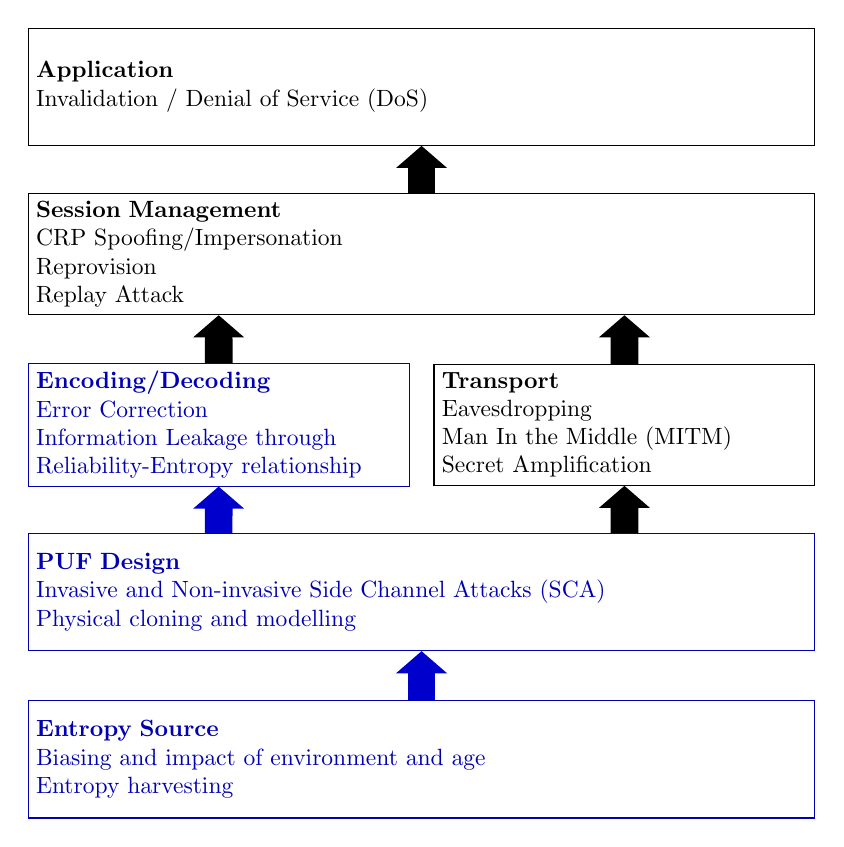
\begin{tikzpicture}[node distance=2.5cm,minimum height=1.75cm, scale=0.85, every node/.style={scale=0.85}]
	\node (source) at (0,0) [shape=rectangle,draw, blue!70!black, text width=.95\linewidth, align=left] {\textbf{Entropy Source}\\Biasing and impact of environment and age\\Entropy harvesting};
	\node (puf) [above of=source, shape=rectangle,draw, blue!70!black, text width=.95\linewidth,align=left] {\textbf{PUF Design}\\Invasive and Non-invasive Side Channel Attacks (SCA)\\Physical cloning and modelling};

	\node (code) [above of=puf, shape=rectangle,draw, blue!70!black, text width=.45\linewidth,align=left,xshift=-.25\linewidth] {\textbf{Encoding/Decoding}\\Error Correction\\Information Leakage through Reliability-Entropy relationship};
	\node (transport) [above of=puf, shape=rectangle,draw, text width=.45\linewidth,align=left,xshift=.25\linewidth] {\textbf{Transport}\\Eavesdropping\\Man In the Middle (MITM)\\Secret Amplification};

	\node (session) [above of=puf, shape=rectangle,draw, text width=.95\linewidth,align=left,yshift=2.55cm] {\textbf{Session Management}\\CRP Spoofing/Impersonation\\Reprovision\\Replay Attack};
	\node (app) [above of=session, shape=rectangle,draw, text width=.95\linewidth,align=left] {\textbf{Application}\\Invalidation / Denial of Service (DoS)};

	\draw [-{Triangle[width=18pt,length=8pt]}, line width=10pt, blue!80!black] (source.north) -- (puf.south);
	\draw [-{Triangle[width=18pt,length=8pt]}, line width=10pt, blue!80!black] ([xshift=-.25\linewidth]puf.north) -- (code.south);
	\draw [-{Triangle[width=18pt,length=8pt]}, line width=10pt] ([xshift=.25\linewidth]puf.north) -- (transport.south);
	\draw [-{Triangle[width=18pt,length=8pt]}, line width=10pt] (code.north) -- ([xshift=-.25\linewidth]session.south);
	\draw [-{Triangle[width=18pt,length=8pt]}, line width=10pt] (transport.north) -- ([xshift=.25\linewidth]session.south);
	\draw [-{Triangle[width=18pt,length=8pt]}, line width=10pt] (session.north) -- (app.south);
\end{tikzpicture}

\end{document}
